\documentclass[utf8,handout]{beamer}
\usepackage{presentation}
\title{Semantic similarity search in Array Express Archive.}
\subtitle{Using experiment metadata}
\author{E. A Tuzova}

\institute{European Bioinformatics institute}
\date{}


\begin{document}

\begin{frame}
  \titlepage
\end{frame}


\section*{Plan}
  \begin{frame}
    \frametitle{Plan}
    \tableofcontents[pausesections]

  \end{frame}

\section{Array Express Archive}
\begin{frame}
	\frametitle{Array Express Archive} 
The ArrayExpress Archive is a database of functional genomics experiments including gene expression where you can query and download data.
\end{frame}

\begin{frame}
	\frametitle{Array Express Archive} 
	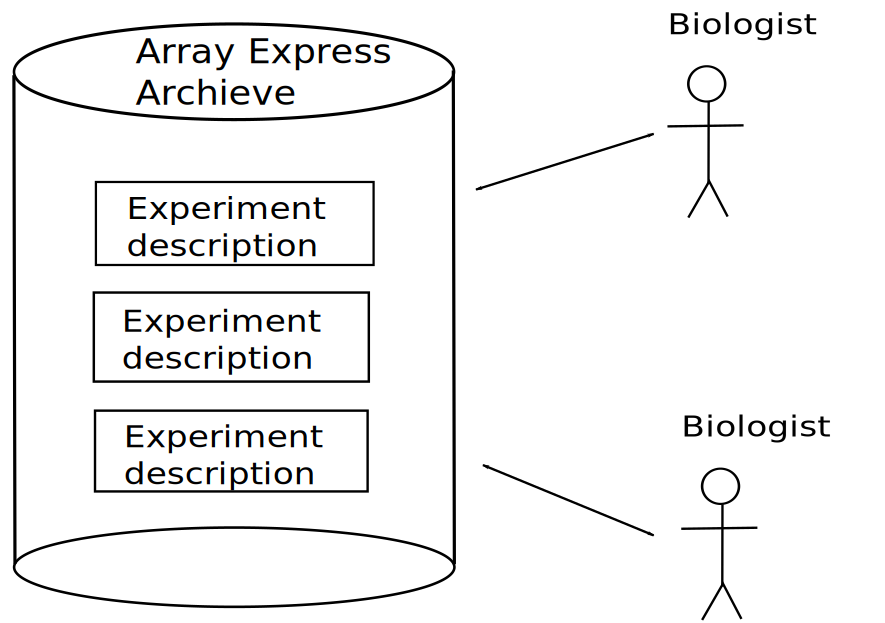
\includegraphics[width=0.6\textwidth]{./arrayExpress}
	\includegraphics[width=0.35\textwidth]{./experimentDescription}	

\end{frame}

\section{Project goals}
  \begin{frame}
    \frametitle{Project goals}
    \begin{block}{}
    	{
    	\Large
    	Project aims to provide information about similar experiments.\\
    	\ \\
    	Save time for real science.}
	\end{block}

  \end{frame}

\section{Possible solutions}
  \begin{frame}

    \frametitle{Possible solutions}
    \begin{enumerate}
      \item Use sample attributes
      \item Use ontology
      \item Use publication references
    \end{enumerate}
  \end{frame}

\section{Sample attributes}
  \begin{frame}
    \frametitle{Sample attributes}  
	\includegraphics[width=0.9\textwidth]{./sampleAttribute}       
  \end{frame}


\section{Zooma}
  \begin{frame}
    \frametitle{Zooma}  
	\includegraphics[width=0.9\textwidth]{./zooma}       
  \end{frame}

\section{Ontology}
  \begin{frame}
    \frametitle{Ontology}  
\begin{flushleft}
	\includegraphics[width=1.4\textwidth]{./ontology}       
\end{flushleft}
  \end{frame}


\section{PubMed articles}
  \begin{frame}
    \frametitle{PubMed articles} 
    http://www.ncbi.nlm.nih.gov/pubmed  \\
    \ \\
	PubMed is a service of the US National Library of Medicine that includes over 19 million citations from MEDLINE and other life science journals.\\

  \end{frame}

  \begin{frame}
    \frametitle{PubMed articles} 
		
\includegraphics[width=0.7\textwidth]{./pubMed}       	
  \end{frame}

\section{Architecture}
  \begin{frame}
    \frametitle{Architecture}  
	\begin{itemize}
		\item Multithreading (Quartz)
		\item Stand-alone modules
	\end{itemize}
  \end{frame}

\section{Properties}
  \begin{frame}
    \frametitle{Properties}  
	\begin{itemize}
		\item amount of similar experiments to store in database
		\item amount of nearest nodes in ontology to use
		\item some properties for publication references
	\end{itemize}
  \end{frame}

  \begin{frame}
		\includegraphics[width=1.3\textwidth]{./ScreenShot_1}       	
  \end{frame}
  \begin{frame}
		\includegraphics[width=1.3\textwidth]{./ScreenShot_2}       	
  \end{frame}
  
  \begin{frame}
		\begin{center}
{
\LARGE{\LARGE{Thank you.}}
}
\end{center}
  \end{frame}
\end{document}